\documentclass[lettersize,journal,12pt]{IEEEtran}
\usepackage{fontspec}
\usepackage{amsmath,amsfonts}
\usepackage{algorithmic}
\usepackage{algorithm}
\usepackage{array}
\usepackage[caption=false,font=normalsize,labelfont=sf,textfont=sf]{subfig}
\usepackage{textcomp}
\usepackage{stfloats}
\usepackage{url}
\usepackage{verbatim}
\usepackage{xeCJK}
\usepackage{lettrine}
\usepackage{graphicx}
\usepackage{titling}
\usepackage{titlesec}
\usepackage{balance}
\usepackage{textcase}
\usepackage{setspace}
\setmainfont{Times New Roman}[SmallCapsFont=TeX Gyre Termes:+smcp]
% rule to break words
\hyphenation{}
\def\BibTeX{{\rm B\kern-.05em{\sc i\kern-.025em b}\kern-.08em
T\kern-.1667em\lower.7ex\hbox{E}\kern-.125emX}}
\pretitle{\begin{center}\fontsize{16}{18}\selectfont\bfseries}
\posttitle{\end{center}}
\preauthor{\begin{center}\fontsize{10}{12}\selectfont}
\postauthor{\end{center}}
\predate{\begin{center}\fontsize{10}{12}\selectfont}
\postdate{\end{center}}
\titleformat{\section}
{\filcenter\fontsize{14}{16}\bfseries\uppercase}
{\thesection}
{1em}
{}
\renewenvironment{abstract}
{\fontsize{12}{14}\textit{\textbf{\abstractname---}}\bfseries\ignorespaces}
{}
\renewenvironment{IEEEkeywords}
{\fontsize{12}{14}\textit{\textbf{Keywords---}}\bfseries\ignorespaces}{}
\begin{document}
\onehalfspacing
\title{Unveiling the PageRank Algorithm: Principles, Performance, and Enhancements}
\author{Wu Zelin, Wu Zekai, Li Pengda}

\maketitle\thispagestyle{headings}
\markboth{10225101428 吴泽霖\quad10225101429 武泽恺\quad10225101460 李鹏达}{}%

\begin{abstract}
	This is the abstract area. We should write a very nb abstract here.
\end{abstract}

\begin{IEEEkeywords}
	Keyword1, Keyword2, Keyword3
\end{IEEEkeywords}


\section{Introduction}

\subsection{Research Background}

\lettrine{W}{ith} 
the proliferation of the Internet technology, the explosively increasing amount of web pages on the World Wide Web has created the demand for the web searching engines with high-efficiency and high-effectiveness. 
For the biggest search engine company Google, which held a global market share of 91.54\% until November 2023\footnote[1]{Search Engine Market Share Worldwide, Statcounter GlobalStats, 2023, https:
//gs.statcounter.com/search-engine-market-share}, it is of primary significance to develop a powerful search algorithm to provide users with the most relevant and useful results in the shortest time. 

\begin{figure}[h]
    \centering
    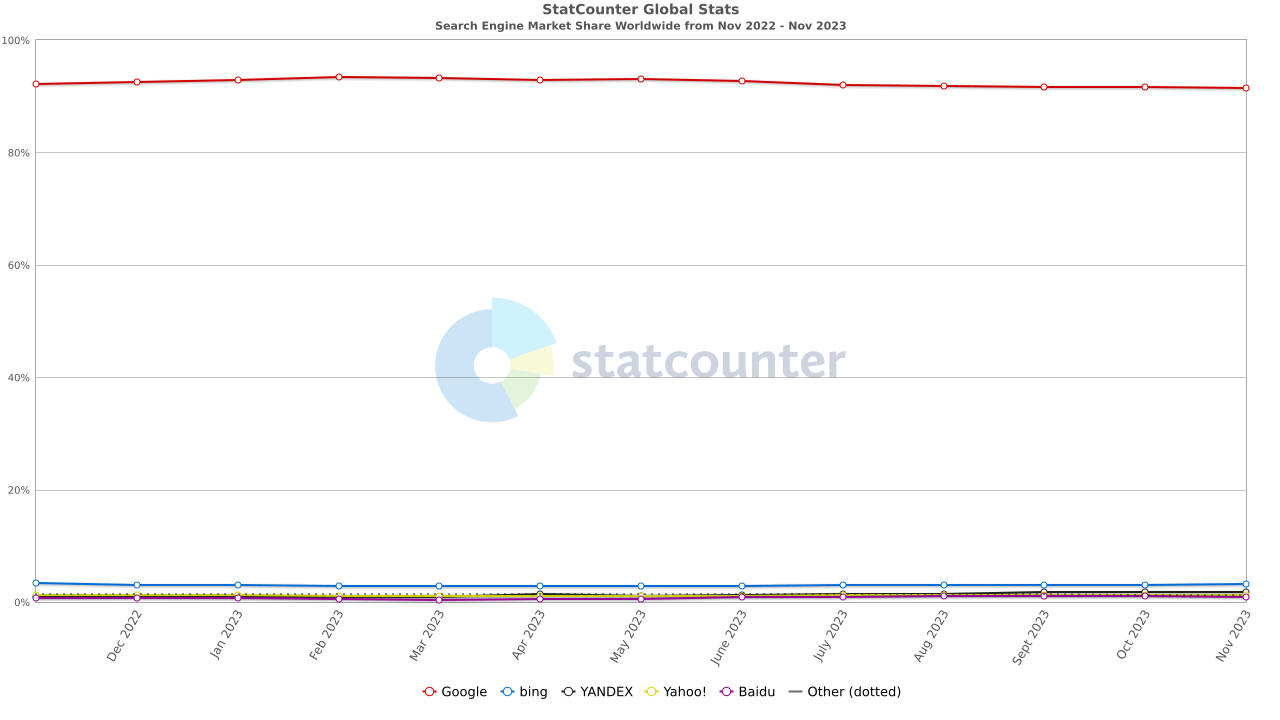
\includegraphics[width=2.5in]{images/fig2.png}
    \caption{Google's market share in the global search engine market from December 2022 to November 2023.}
    \label{fig1}
\end{figure}

Previous studies on web searching algorithms have proven that TF-IDF algorithm and BM25 algorithm were efficient and effective in the early days of the Internet.

However, these algorithms have been unable to meet the growing demand of users.
The users' search queries are becoming diversified and the web pages are becoming complex.
According to the statistics, the amount of web pages, a 130-fold increase over 20 years, has surged to 130 trillion in 2016, which means it takes much longer time to search for the most relevant web pages.
To overcome the aformentioned chanllenge, Google has developed a state-of-the-art algorithm called PageRank, which is currently a fundamental algorithm in web search, redefining how we navigate web search.

\subsection{Origin of the PageRank Algorithm} 
PageRank is an algorithm developed by Larry Page and Sergey Brin in the late 1990s to measure the importance of web pages. 
Originally created for the Google search engine, it is named after one of the founder of Google Larry Page. Except for the searching use, the Google search engine also takes advantage of this algorithm to analyze the relevance and importance of web pages, considering it as one of the factors to evaluate the effectiveness of web page optimization. 

\subsection{Outline of this Paper}

In this paper, we present the following insights and research:
\begin{itemize}
	\item The foundational principles and implementation of the PageRank algorithm.(Section 3, Subsection A)
	\item Analysis of its performance and the impact of the factors that can influence the search results and page rankings.(Section 4, Subsection A)
	\item Discussion on potential enhancements and exploration of the possibility of other factors that can improve PageRank performance.(Section 4, Subsection B)
\end{itemize}

In the next section, we introduce the preliminaries and the related work of the PageRank algorithm.

\section{Related Work}

These section shows the brief concept of the PageRank algorithm. Theses concept motivate the design of our research.

\subsection{TF-IDF Algorithm}


\subsection{Synopsis of PageRank}

PageRank is a link analysis algorithm and it assigns a numerical weighting to each web page of all hyperlinked web pages, aiming to measure the relative importance of each web page of the collection based on its parent web page's importance. This algorithm can be applied to any collection containing mutual references between elements.We call the weight value of any element E as ``PageRank of E", which is represented symbolically as $\boldsymbol{PR(E)}$. Other factors such as ``Author Rank" can also affect the weight value of an element.

A PageRank results from a mathematical algorithm based on the webgraph, created by all World Wide Web pages as nodes and hyperlinks as edge, taking into consideration anthority hubs such as CNN. The rank value indicates an importance of a particular page. A hyperlink to this web page is called ``a vote of support for this web page". The weight of each web is defined recursively, based on the weight of all pages linking to it. For example, a page linked to many pages will have a high PageRank.

Many academic papers on PageRank existed before Page and Brin's original paper. In actual situations, PageRank is easily exploited. Relevant research tends to focus on those PageRank results affected by errors. In order to solve the problem, Google launched a new attribute nofollow for web links. The attribute allows webmasters and blogger to create some links that do not count, which means that these links do not serve as the ``vote'' so that they can ignore the spam votes.

\subsection{Markov Chain}

Markov chain, also called discrete-time Markov chain, is named after the Russian mathematician Andrei Markov. The chain is a random process in state space that undergoes a transition from a state to another. The process requires ``memoryless'' properties. That means the probability distribution of the next state can only be determined by the current state. Simultaneously, the previous events in the time series have no connection with it. The specific type of ``memoryless'' is called Markov properties. Markov chains have many applications as statistical models of real process.

At each step of the Markov chain, the system can maintain or change from one state to another according to the probability distribution. State changes are called transitions, and the probabilities associated with different state changes are called transition probabilities.

If the Markov chain runs for enough time, the distribution of its state will reach a stationary distribution and remain unchanged. Formally, if the Markov chain has $n$ states, the transition matrix is $P$
, and the stationary distribution vector is $\boldsymbol{\pi}$, then $\boldsymbol{\pi} = \boldsymbol{\pi} P$ is satisfied.

This means that the stationary distribution vector $\boldsymbol{\pi}$ is an eigenvector of the transfer matrix $P$ and corresponds to an eigenvalue of 1. Specifically, a stationary distribution has the following properties:
\begin{enumerate}
	\item [1.] $\boldsymbol{\pi_i}\geq0$, and $\sum\boldsymbol{\pi_i}=1$. That is, each element of a stationary distribution is non-negative and sums to 1, representing probability.
	\item [2.] $\boldsymbol{\pi} = \boldsymbol{\pi} P$. That is, the stationary distribution vector is the eigenvector of the transfer matrix, and the corresponding eigenvalue is 1. This shows that if the current state is stationary, then after one step of transition, the state distribution will still be stationary.
	\item [3.] Do not depend on initial state. No matter what the initial state is, after a long enough transfer, the Markov chain
	      The state distribution will reach a stationary distribution.
	\item [4.] Uniqueness. The stationary distribution of a Markov chain is unique.
\end{enumerate}

Stationary distribution represents the stable state of the Markov chain after long-term operation and will no longer be affected by the initial state.
It measures the frequency of each state in the entire chain, giving the Markov chain stable operation of each
the proportion of time spent in the state.

Assumeing that when we browse a page on the Internet, the process of selecting the next interface has no collection with that we browse before but only depends on the current page. This is a simple finite-state, discrete-time stochastic process that can be described using a Markov chain.

\subsection{PageRank Algorithm and Eigenvalues of  Matrix}

The PageRank algorithm is related to the eigenvalue of the matrix. Before the PageRank algorithm was proposed, eigenvalue of the matrix questions are used in many problems. Many have independently proposed using eigenvalue problems, including Edmund Landau's proposal(1895) for determining the winner of a chess tournament, Gabriel Pinski and Francis Narin's work(1976) on ranking scientific journals in scientometrics, Thomas Saaty's work(1977) on the weighted alternative choice, Bradley Love and StevenSloman's work on a cognitive model, namely the centrality algorithm. 

\section{Main Method and Theory}

\subsection{Foundational principles}




We can make a citation here. \cite{ref1}

% \figurename~\ref{fig2} is a figure. You can see it at the top of the page.

% \begin{figure}[!t]
% 	\centering
% 	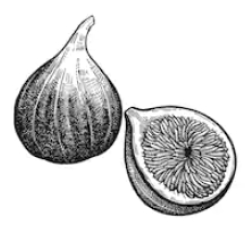
\includegraphics[width=2.5in]{images/fig1.png}
% 	\caption{This is a figure.}
% 	\label{fig2}
% \end{figure}

\subsection{The 3rd Section 2nd Subsection}

This is a simple subsection too.
\section{Experiment}

This is a simple section.
\subsection{The 4th Section 1st Subsection}

This is a simple subsection.

This is an equation:

\begin{equation}
	\label{eq:1}
	e^{\pi i} + 1 = 0
\end{equation}
You can ref it by see\eqref{eq:1}.

\subsection{The 4th Section 2nd Subsection}

This is a simple subsection too.

This is a algorithm:

\begin{algorithm}[H]
	\caption{Weighted Tanimoto ELM.}\label{alg:alg1}
	\begin{algorithmic}
		\STATE
		\STATE {\textsc{TRAIN}}$(\mathbf{X} \mathbf{T})$
		\STATE \hspace{0.5cm}$ \textbf{select randomly } W \subset \mathbf{X}  $
		\STATE \hspace{0.5cm}$ N_\mathbf{t} \gets | \{ i : \mathbf{t}_i = \mathbf{t} \} | $ \textbf{ for } $ \mathbf{t}= -1,+1 $
		\STATE \hspace{0.5cm}$ B_i \gets \sqrt{ \textsc{max}(N_{-1},N_{+1}) / N_{\mathbf{t}_i} } $ \textbf{ for } $ i = 1,...,N $
		\STATE \hspace{0.5cm}$ \hat{\mathbf{H}} \gets  B \cdot (\mathbf{X}^T\textbf{W})/( \mathbb{1}\mathbf{X} + \mathbb{1}\textbf{W} - \mathbf{X}^T\textbf{W} ) $
		\STATE \hspace{0.5cm}$ \beta \gets \left ( I/C + \hat{\mathbf{H}}^T\hat{\mathbf{H}} \right )^{-1}(\hat{\mathbf{H}}^T B\cdot \mathbf{T})  $
		\STATE \hspace{0.5cm}\textbf{return}  $\textbf{W},  \beta $
		\STATE
		\STATE {\textsc{PREDICT}}$(\mathbf{X} )$
		\STATE \hspace{0.5cm}$ \mathbf{H} \gets  (\mathbf{X}^T\textbf{W} )/( \mathbb{1}\mathbf{X}  + \mathbb{1}\textbf{W}- \mathbf{X}^T\textbf{W}  ) $
		\STATE \hspace{0.5cm}\textbf{return}  $\textsc{sign}( \mathbf{H} \beta )$
	\end{algorithmic}
	\label{alg1}
\end{algorithm}

\section{Results}

This is the results area. We should write some very nb results here.

\section{Conclusion}

This is the conclusion area. We should write a very nb conclusion here.



\begin{thebibliography}{1}

	\bibitem{ref1}
	S. Zhan, S. Li and W. Wang, {\it{A Very Nb Book}}. Shanghai, P.R.C., East China Normal  Univ. Press, 2022.

\end{thebibliography}

\end{document}


